\clearpage
\section{Аппроксимация спектров инвариантных масс}
\label{sec:fitting}

Характеристики распадов и резонансов извлекаются из спектров 
инвариантных масс частиц конечного состояния. Для этого строятся 
функции, зависящие от нескольких параметров, и производится 
аппроксимация спектров, позволяющая определить значения и погрешности 
вычисления параметров модели. Для успешной и точной обработки данных 
необходимо учесть все особенности распределения масс и все процессы, 
дающие вклад в его формирование.

\label{sec:fitting:lb-dppipi}

Спектр инвариантных масс $m(\Dp\p\pim\pim)$ обладает узким пиком, 
соответствующим распаду $\Lb\to\Dp\p\pim\pim$ и широкой структурой слева 
от основного пика, соответствующей распаду через резонансное состояние 
$\Lb\to\Dstarp\p\pim\pim$. Мезон $\Dstarp$ в этом случае распадается на 
$\Dp\piz$ или $\Dp\gamma$, где нейтральная частица не восстанавливается 
детектором. Фон в спектре масс состоит из двух компонент. Во-первых, 
в него входят случайные комбинации треков, удовлетворяющие всем 
критериям отбора событий. Эта компонента называется комбинаторным фоном. 
Во-вторых, помимо распада через резонанс $\Dstarp$, барион $\Lb$ может 
испытывать прямой распад на конечное состояние $\Dp\piz\p\pim\pim$. Как 
будет показано далее, этот вклад имеет форму, не обладающую выраженным 
пиком и, кроме того, не подлежит изучению в данном анализе и поэтому 
считается частью фона. Прямой распад на состояние $\Dp\gamma\p\pim\pim$ 
тоже возможен, но не учитывается, поскольку его вероятность существенно 
меньше адронной моды, а смысла в увеличении количества параметров фона 
нет.

Форма вклада, описывающего распад $\Lb\to\Dp\pim\pim$, представляет 
собой чистую реакцию детектора и алгоритмов восстановления треков, 
поскольку все частицы в конечном состоянии заряженные и успешно 
регистрируются, а естественная ширина $\Lb$ имеет чрезвычайно малую 
величину $\Gamma_\Lb\rep{\approx} \hbar/\tau_\Lb\rep{\approx} 
4.5\cdot10^{-4}$~эВ~\cite{PDG}, обусловленную тем, что распад происходит 
по слабому взаимодействию.
%
Во многих ситуациях отклик детектора можно считать гауссовым, но, 
с учетом описанных обстоятельств и важности рассматриваемой компоненты, 
распределение Гаусса недостаточно точно воспроизводит данные 
эксперимента, особенно при б\'{о}льших отклонениях от центрального 
значения пика. Среди процессов, происходящих при регистрации частиц и не 
подчиняющихся распределению Гаусса, также можно назвать потери энергии 
до входа в калориметры.
%
Для учета этих факторов была выбрана следующая функция:
\[%Dp signal mode{{{
  S_{\Dp} = N\cdot
  \begin{cases}
    \exp\left(-\frac{(m-m_0)^2}{2\sigma_m^2}\right), &
    -\alpha_L < \frac{m-m_0}{\sigma_m} < \alpha_R, \\
    A_L\cdot\left(B_L - \frac{m-m_0}{\sigma_m}\right)^{-n_L},
    & \frac{m-m_0}{\sigma_m} \leq -\alpha_L, \\
    A_R\cdot\left(B_R + \frac{m-m_0}{\sigma_m}\right)^{-n_R},
    & \frac{m-m_0}{\sigma_m} \geq \alpha_R, 
  \end{cases}
\]%}}}
в которой $m = m(\Dp p\pim\pim)$; $\alpha_L$, $\alpha_R$, $n_L$, $n_R$, 
$m_0$, $\sigma_m$ -- параметры аппроксимации, каждый из которых больше 
нуля, а $n_L,\,n_R>1$. Коэффициенты $A_L$, $A_R$, $B_L$, $B_R$, $N$ 
находятся из условий нормировки $S_{\Dp}$ на единицу и непрерывности 
$S_{\Dp}(m)$ и ее производной:
\[\begin{aligned}%normalization and smoothness{{{
  A_{L,R} \,&= \left(\frac{n_{L,R}}{\alpha_{L,R}}\right)^{n_{L,R}}
  \cdot \exp\!\left({-\frac{\alpha_{L,R}^2}{2}}\right), \\ 
B_{L,R} \,&= \frac{n_{L,R}}{\alpha_{L,R}} - \alpha_{L,R}, \\ 
N \,&= \frac{1}{\sigma_m} \, \frac{1}{I_L + I_R}, \\
I_{L,R} \,&= \sqrt{\frac{\pi}{2}}\,\erf{\frac{\alpha_{L,R}}{\sqrt{2}} } + 
\frac{1}{\alpha_{L,R}}\,\frac{n_{L,R}}{n_{L,R}-1}\,\exp\!\left({-\frac{\alpha_{L,R}^2}{2}}\right).
\end{aligned}\]%}}}
Функция подобного вида, но со степенным хвостом только с одной стороны, 
была впервые рассмотрена участником коллаборации Crystal 
Ball~\cite{CrystalBall-function} и называется Crystal Ball функцией. 
Сравнение двухсторонней Crystal Ball функции с традиционным 
распределением Гаусса от переменной $x=\frac{m-m_0}{\sigma_m}$ для 
иллюстративного набора параметров показано на 
рисунке~\ref{fig:crystalball}.

\begin{figure}%crystal ball{{{
  \centering
  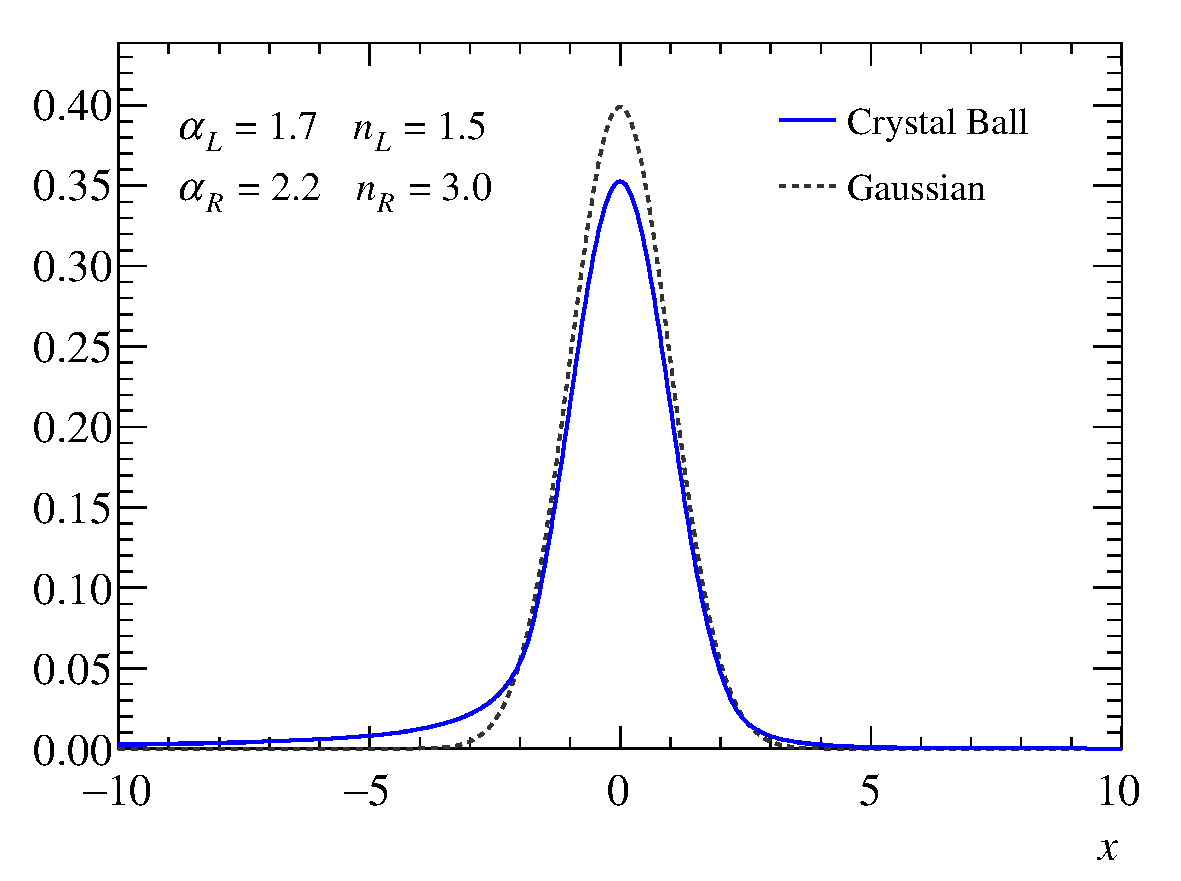
\includegraphics[width=.5\linewidth]{figures/crystalball}
  \caption{Сравнение выбранной модели распада $\Lb\to\Dp\p\pim\pim$ 
  с функцией Гаусса для иллюстративного набора параметров.}
  \label{fig:crystalball}
\end{figure}%}}}

Для резонансного распада $\Lb\to\Dstarp\p\pim\pim$ при 
$\Dstarp\to\Dp\piz\ /\ \Dp\gamma$ и прямого распада 
$\Lb\to\Dp\piz\p\pim\pim$ пользоваться функцией отклика детектора 
напрямую невозможно, поскольку в каждом из них одна из частиц в конечном 
состоянии имеет нулевой заряд и в данном анализе не восстанавливается. 
Для их аппроксимации используется следующий подход. Сперва, с помощью 
метода Монте-Карло производится моделирование распадов и извлекаются 
распределения событий по массе $m(\Dp\p\pim\pim)$, обусловленные 
кинематикой. Результаты этого этапа представлены на 
рисунке~\ref{fig:dstar-dpiz-simulation}. Затем, для учета влияния 
детектора и процесса реконструкции событий полученные распределения 
сворачиваются с функцией Гаусса с нулевым средним и шириной, взятой из 
гауссовой основы модели канала $\Lb\to\Dp\p\pim\pim$, описанной ранее. 
Кроме того, для компенсации неточности, вносимой разницей в кинематике 
распада $\Lb\to\Dstarp\p\pim\pim$ в симуляции и в эксперименте, 
полученные для $\Dstarp$ распределения модулируются полиномом первой 
степени со свободными параметрами. Модулировать спектр прямого распада 
через $\Dp\piz$ не имеет смысла, поскольку фон в этой области не 
нуждается в дополнительных параметрах. Полученные в итоге функции далее 
обозначены как $S_{\Dstarp(\piz)}$, $S_{\Dstarp(\gamma)}$ 
и~$S_{\Dp\piz}$.

\begin{figure}%dstar-dpiz-simulation{{{
  \centering
  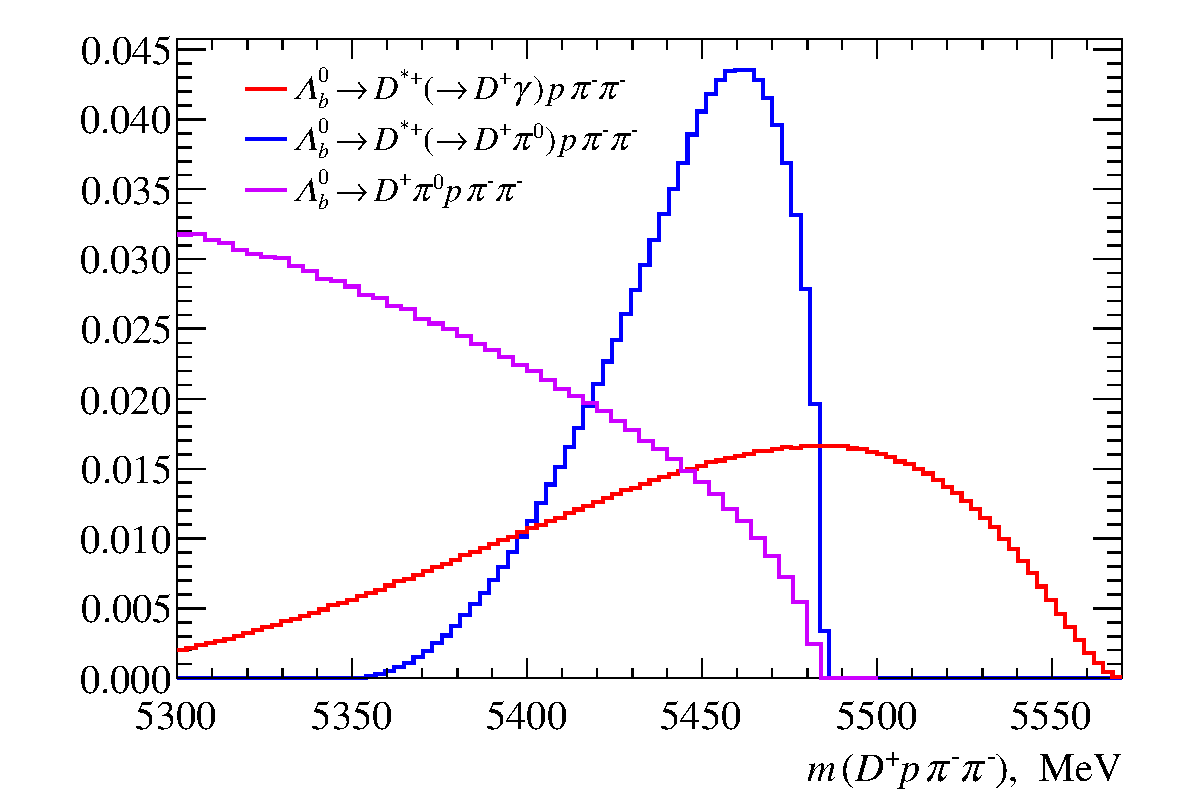
\includegraphics[width=.5\linewidth]{figures/dstar-dpiz-simulation}
  \caption{Распределения инвариантных масс $m(\Dp\p\pim\pim)$ распадов 
  \mbox{$\Lb\to\Dstarp\p\pim\pim$} и $\Lb\to\Dp\piz\p\pim\pim$, обусловленные 
  кинематикой.}
  \label{fig:dstar-dpiz-simulation}
\end{figure}%}}}

Для более точного извлечения параметров, описывающих модель распада 
$\Lb\to\Dstarp\p\pim\pim$, необходимо принять во внимание два фактора. 
Во-первых, компонента, соответствующая моде $\Dstarp\to\Dp\gamma$ не 
имеет ярко выраженного пика даже до учета отклика детектора и тем более 
не будет иметь после. Во-вторых, названная мода реализуется 
электромагнитным взаимодействием, а конкурирующая -- сильным, вследствие 
чего интегральное количество соответствующих ей событий ожидается 
довольно малым. Для компенсации этих недостатков вклады двух распадов 
через промежуточное состояние с резонансом $\Dstarp$ складываются 
с коэффициентами, учитывающими вероятности этих мод: 
$\BR{\Dstarp\to\Dp\piz} = 30.7 \pm 0.5 \%$, $\BR{\Dstarp\to\Dp\gamma} 
= 1.6 \pm 0.4 \%$~\cite{PDG}. В результате модель вклада канала 
$\Lb\to\Dstarp\p\pim\pim$ приобретает вид
\[ S_{\Dstarp} = \alpha S_{\Dstarp(\piz)} + \beta S_{\Dstarp(\gamma)},
\qquad \beta/\alpha = 0.052 \pm 0.013.\]
Наличие погрешности у отношения вероятностей мод распада $\Dstarp$ 
приводит к неоднозначности выбора коэффициентов сложения, а вместе 
с этим и к систематической ошибке. Она вычисляется отдельно.

Комбинаторный фон имеет гладкую монотонную форму и описывается убывающим 
полиномом третьей степени.

Кроме того, для увеличения точности извлекаемых из экспериментальных 
данных результатов общепринятой практикой является фиксирование 
определенных параметров модели на значениях, полученных при 
аппроксимации более обширных наборов данных эксперимента или же 
моделирования. Если не фиксировать такие параметры, погрешность 
результатов, обусловленная конечностью набора данных и называемая 
статистической, будет существенно увеличена благодаря их вариации. 
С другой стороны, при фиксации этих параметров появляются дополнительные 
``входные данные'' модели. Выбор значений, на которых они фиксируются, 
во-первых, должен быть строго обоснован, а во-вторых, никогда не может 
быть единственным. Таким образом, возникает погрешность, обусловленная 
способом обработки данных, то есть систематическая. Как видно, 
определенная ошибка присутствует в обоих подходах, но складывается из 
разных компонент. Если во втором подходе удается достаточно сильно 
ограничить разумные пределы изменения таких параметров, систематическая 
погрешность может оказаться меньше статистической первого подхода. 
В этом случае выгодно воспользоваться описанной процедурой. В данной 
работе такой подход реализован для параметров $\alpha_{L,R}$, $n_{L,R}$ 
степенных хвостов модели распада $\Lb\to\Dp\p\pim\pim$: их величины 
фиксируются на значениях, полученных при аппроксимации данных 
моделирования.

Полная модель спектра масс $m(\Dp\p\pim\pim)$ является суммой всех 
описанных вкладов с варьируемыми коэффициентами -- числами событий, 
которые и представляют наибольший интерес. Для нахождения этих чисел 
и всех остальных параметров модели минимизируется логарифм расширенной 
функции правдоподобия, взятый с противоположным 
знаком~\cite{extended-likelihood}
\[\begin{aligned}%{{{
  -\mathrm{log}\mathcal{L} =& -\sum\limits_{k=1}^{N_\text{полн}}
  \mathrm{log}\left(N_\Dp S_\Dp + N_\Dstarp S_\Dstarp + N_{\Dp\piz}
               S_{\Dp\piz} + N_\text{фон} B\right) + \\
  & + \left(N_\Dp + N_\Dstarp + N_{\Dp\piz} + N_\text{фон}\right) - \\
  & - N_\text{полн}\,\mathrm{log}\left(N_\Dp + N_\Dstarp + N_{\Dp\piz}
                                  + N_\text{фон}\right),
\end{aligned}\]%}}}
где $N_i$ -- число событий во вкладе $i$, $S_i$ -- его модель, $B$ -- 
модель фона, а $N_\text{полн}$ -- полное число наблюдаемых событий 
в спектре. При минимизации наборы данных не разбиваются по ячейкам на 
оси, а сохраняются в виде точек. Результат аппроксимации 
экспериментального спектра в проекции на распределение по ячейкам 
показан на рисунке~\ref{fig:lb-dppipi-fit}, а значения основных 
параметров приведены в таблице~\ref{tab:lb-fit-results}. Этот результат 
был опубликован в статье~\cite{lb2dppipi-paper}.

\begin{figure}[t!]%lb-dppipi-fit{{{
  \centering
  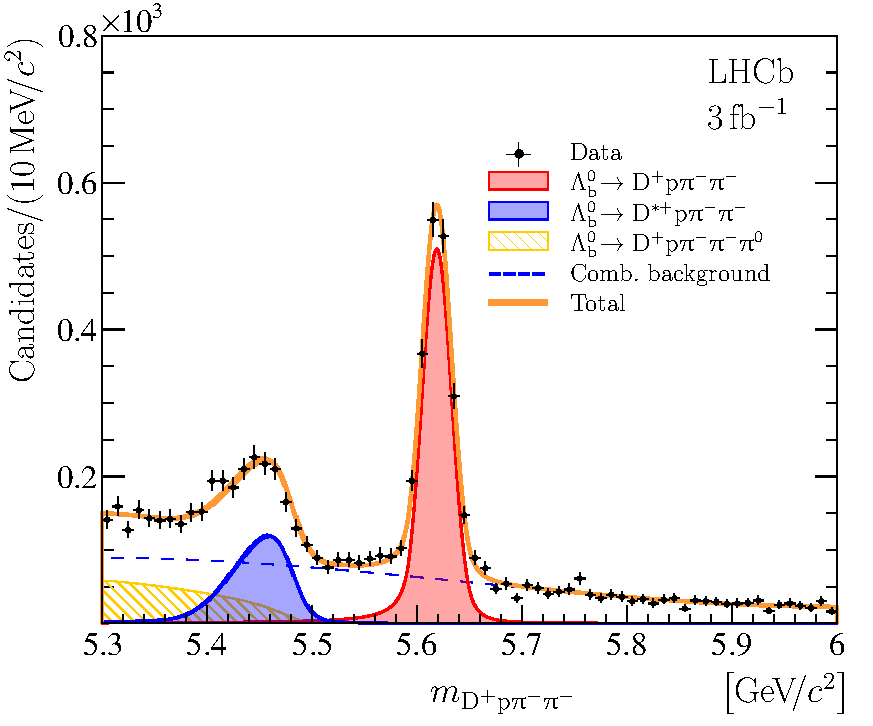
\includegraphics[width=.5\linewidth]{figures/lb-dppipi-fit}%
  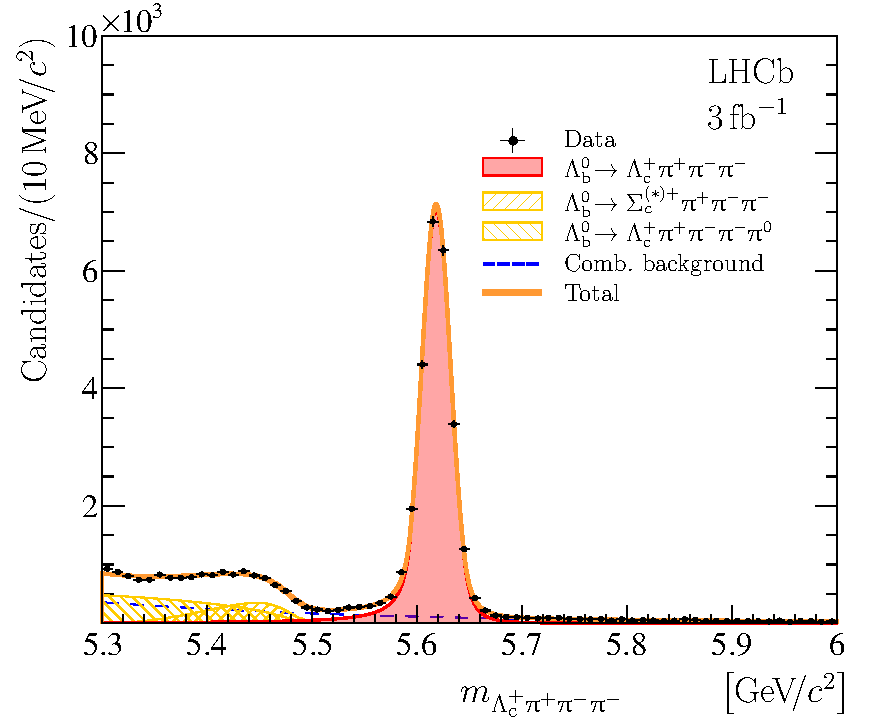
\includegraphics[width=.5\linewidth]{figures/lb-lc3pi-fit}
  \caption{Аппроксимация экспериментальных спектров инвариантных масс 
  $m(\Dp\p\pim\pim)$ и $m(\Lc\pip\pim\pim)$~\cite{lb2dppipi-paper}.}
  \label{fig:lb-dppipi-fit}
  \label{fig:lb-lc3pi-fit}
\end{figure}%}}}

\begin{table}[b!]%lb-fit-results{{{
  \centering
  \caption{Основные результаты аппроксимации экспериментальных спектров 
  инвариантных масс $m(\Dp\p\pim\pim)$ и $m(\Lc\pip\pim\pim)$.}
  \label{tab:lb-fit-results}
  \begin{tabular}{|c|c|c|c|}
    \hline
    Параметр & Значение & Параметр & Значение \\
    \hline
    $N_\Dp$        & $1933 \pm  56$ &  $N_\Lc$        & $26505 \pm 177$\\
    $N_\Dstarp$    & $ 862 \pm  55$ &  $N_\Scoptstarp$& $ 3301 \pm 130$\\
    $N_{\Dp\piz}$  & $ 674 \pm 209$ &  $N_{\Lc\piz}$  & $ 6234 \pm 285$\\
    \hline
  \end{tabular}
\end{table}%}}}

\begingroup \par \sloppy
Спектр инвариантных масс $m(\Lc\pip\pim\pim)$ имеет схожую структуру, 
составляемую распадами $\Lb\to\Lc\pip\pim\pim$, 
$\Lb\to\Scoptstarp\pip\pim\pim$ при \mbox{$\Scoptstarp\to\Lc\piz$}, 
$\Lb\to\Lc\piz\pip\pim\pim$ и комбинаторным фоном. Аналогично модели 
спектра $m(\Dp\p\pim\pim)$, распад $\Lb\to\Lc\pip\pim\pim$ описывается 
Crystal Ball функцией, вклады распадов, в конечных состояниях которых 
присутствует нейтральный пион, определяются из Монте-Карло моделирования 
и сворачиваются с гауссианом, а комбинаторный фон моделируется убывающим 
полиномом третьей степени. Параметры хвостов Crystal Ball функции, как 
и прежде, фиксируются на значениях, полученных при аппроксимации данных 
моделирования. Результат аппроксимации экспериментального спектра 
$\Lc\pip\pim\pim$ представлен на рисунке~\ref{fig:lb-lc3pi-fit}~слева, 
а значения основных параметров приведены 
в таблице~\ref{tab:lb-fit-results}. Этот результат также опубликован 
в статье~\cite{lb2dppipi-paper}.
\par \endgroup
